% Sketch output, version 0.3 (build 7d, Sun Mar 20 14:11:05 2016)
% Output language: PGF/TikZ,LaTeX
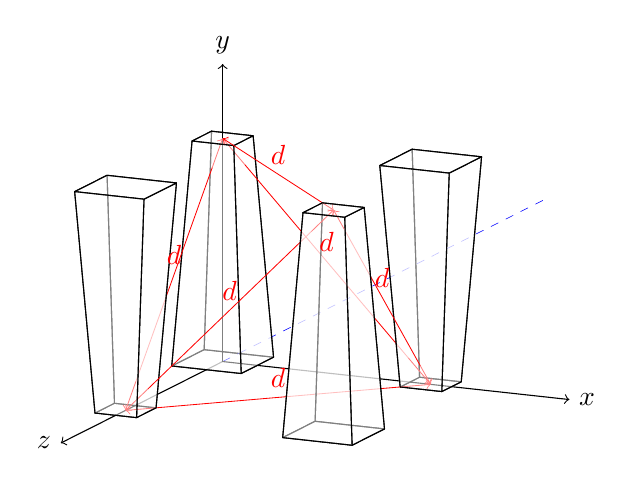
\begin{tikzpicture}[line join=round]
\draw[arrows=-](-2.055,-1.034)--(-2.261,-1.138);
\filldraw[fill opacity=0.5,fill=white](-2.29,-.883)--(-2.701,-1.09)--(-1.82,-1.186)--(-1.409,-.979)--cycle;
\draw[line width=.2pt,draw=blue,dashed](-1.85,-.931)--(2.055,1.034);
\filldraw[fill opacity=0.5,fill=white](-1.409,-.979)--(-2.29,-.883)--(-2.196,1.891)--(-1.668,1.833)--cycle;
\filldraw[fill opacity=0.5,fill=white](-2.29,-.883)--(-2.701,-1.09)--(-2.443,1.767)--(-2.196,1.891)--cycle;
\draw[line width=.2pt,draw=blue,dashed](-2.055,-1.034)--(-1.85,-.931);
\draw[arrows=-](-2.055,-1.034)--(-1.615,-1.083);
\draw[line width=.3pt,arrows=<-,draw=red](-2.055,1.8)--(-1.772,1.465);
\filldraw[fill opacity=0.5,fill=white](-1.82,-1.186)--(-1.409,-.979)--(-1.668,1.833)--(-1.914,1.709)--cycle;
\draw[arrows=-](-2.055,-1.034)--(-2.055,1.8);
\filldraw[fill opacity=0.5,fill=white](.975,-1.291)--(.728,-1.415)--(.2,-1.357)--(.446,-1.233)--cycle;
\draw[arrows=-](-1.615,-1.083)--(.323,-1.295);
\draw[line width=.3pt,arrows=->,draw=red](-2.187,1.43)--(-2.055,1.8);
\filldraw[fill opacity=0.5,fill=white](-2.701,-1.09)--(-1.82,-1.186)--(-1.914,1.709)--(-2.443,1.767)--cycle;
\filldraw[fill opacity=0.5,fill=white](-2.196,1.891)--(-2.443,1.767)--(-1.914,1.709)--(-1.668,1.833)--cycle;
\draw[arrows=-](-2.261,-1.138)--(-3.165,-1.593);
\draw[arrows=->](-2.055,1.8)--(-2.055,2.745);
\draw[line width=.3pt,arrows=<-,draw=red](-2.055,1.8)--(-1.914,1.709);
\draw[line width=.3pt,arrows=-,draw=red](-1.772,1.465)--(.304,-.989);
\filldraw[fill opacity=0.5,fill=white](-.059,1.455)--(.352,1.662)--(.446,-1.233)--(.2,-1.357)--cycle;
\filldraw[fill opacity=0.5,fill=white](.352,1.662)--(1.233,1.566)--(.975,-1.291)--(.446,-1.233)--cycle;
\draw[line width=.3pt,arrows=-,draw=red](-3.156,-1.285)--(-2.187,1.43);
\draw[line width=.3pt,arrows=-,draw=red](-1.914,1.709)--(-.787,.981);
\draw[arrows=-](.323,-1.295)--(.851,-1.353);
\filldraw[fill opacity=0.5,fill=white](1.233,1.566)--(.822,1.359)--(.728,-1.415)--(.975,-1.291)--cycle;
\draw[line width=.3pt,arrows=->,draw=red](.304,-.989)--(.587,-1.324);
\draw[line width=.3pt,arrows=<-,draw=red](.587,-1.324)--(.2,-1.357);
\draw[line width=.3pt,arrows=<-,draw=red](.587,-1.324)--(.455,-1.087);
\filldraw[fill opacity=0.5,fill=white](1.233,1.566)--(.822,1.359)--(-.059,1.455)--(.352,1.662)--cycle;
\draw[arrows=->](.851,-1.353)--(2.349,-1.517);
\filldraw[fill opacity=0.5,fill=white](.822,1.359)--(-.059,1.455)--(.2,-1.357)--(.728,-1.415)--cycle;
\filldraw[fill opacity=0.5,fill=white](-2.901,-1.622)--(-3.148,-1.746)--(-3.676,-1.688)--(-3.429,-1.564)--cycle;
\draw[line width=.3pt,arrows=-,draw=red](.2,-1.357)--(-2.901,-1.622);
\draw[line width=.3pt,arrows=-,draw=red](.455,-1.087)--(-.514,.652);
\filldraw[fill opacity=0.5,fill=white](-3.523,1.331)--(-2.642,1.234)--(-2.901,-1.622)--(-3.429,-1.564)--cycle;
\filldraw[fill opacity=0.5,fill=white](-3.934,1.124)--(-3.523,1.331)--(-3.429,-1.564)--(-3.676,-1.688)--cycle;
\draw[arrows=-](-3.165,-1.593)--(-3.412,-1.717);
\draw[line width=.3pt,arrows=<-,draw=red](-3.288,-1.655)--(-3.156,-1.285);
\draw[line width=.3pt,arrows=->,draw=red](-2.901,-1.622)--(-3.288,-1.655);
\draw[line width=.3pt,arrows=->,draw=red](-3.005,-1.383)--(-3.288,-1.655);
\filldraw[fill opacity=0.5,fill=white](-2.642,1.234)--(-3.054,1.028)--(-3.148,-1.746)--(-2.901,-1.622)--cycle;
\filldraw[fill opacity=0.5,fill=white](-2.642,1.234)--(-3.054,1.028)--(-3.934,1.124)--(-3.523,1.331)--cycle;
\filldraw[fill opacity=0.5,fill=white](-3.054,1.028)--(-3.934,1.124)--(-3.676,-1.688)--(-3.148,-1.746)--cycle;
\filldraw[fill opacity=0.5,fill=white](0,-1.89)--(-.881,-1.793)--(-.787,.981)--(-.258,.923)--cycle;
\draw[line width=.3pt,arrows=-,draw=red](-.929,.617)--(-3.005,-1.383);
\draw[arrows=->](-3.412,-1.717)--(-4.111,-2.069);
\filldraw[fill opacity=0.5,fill=white](-.881,-1.793)--(-1.292,-2)--(-1.034,.857)--(-.787,.981)--cycle;
\filldraw[fill opacity=0.5,fill=white](-.881,-1.793)--(-1.292,-2)--(-.411,-2.097)--(0,-1.89)--cycle;
\filldraw[fill opacity=0.5,fill=white](-.411,-2.097)--(0,-1.89)--(-.258,.923)--(-.505,.799)--cycle;
\draw[line width=.3pt,arrows=->,draw=red](-.514,.652)--(-.646,.89);
\draw[line width=.3pt,arrows=<-,draw=red](-.646,.89)--(-.929,.617);
\filldraw[fill opacity=0.5,fill=white](-1.292,-2)--(-.411,-2.097)--(-.505,.799)--(-1.034,.857)--cycle;
\draw[line width=.3pt,arrows=->,draw=red](-.787,.981)--(-.646,.89);
\filldraw[fill opacity=0.5,fill=white](-.787,.981)--(-1.034,.857)--(-.505,.799)--(-.258,.923)--cycle;
\node[right] at (2.349,-1.517) {$x$};\node[above] at (-2.055,2.745) {$y$};\node[left] at (-4.111,-2.069) {$z$};\node[above,color=red] at (-1.351,1.345) {$d$};\node[above,color=red] at (-1.351,-1.49) {$d$};\node[above,color=red] at (-.734,.238) {$d$};\node[above,color=red] at (-.029,-.217) {$d$};\node[above,color=red] at (-1.967,-.383) {$d$};\node[above,color=red] at (-2.672,.072) {$d$};\end{tikzpicture}% End sketch output
